\documentclass{report}
\usepackage[spanish]{babel}
\usepackage[left=2.5cm, right=2.5cm, top=3cm, bottom=3cm]{geometry}
\usepackage{enumerate}
\usepackage{graphicx}
\usepackage{booktabs}
\usepackage{tabularx}
\usepackage{enumitem}
\usepackage{amsmath}
\usepackage{amsfonts}
\usepackage{float}
\usepackage{hyperref}  
\usepackage{algorithm}
\usepackage{algpseudocode}

% Eliminar numeración del primer nivel (0.)
\renewcommand{\thesection}{\arabic{section}}

% Configurar profundidad máxima de 2 niveles (section, subsection)
\setcounter{secnumdepth}{2}

\title{}
\author{}

\begin{document}

\begin{titlepage}
    \centering
    {\bfseries\LARGE Facultad de Matemática y Computación \par}
    \vfill
    {\scshape\LARGE Simulación \par}
    \vfill
    {\LARGE \textbf{Informe: Simulación del inventario de una tienda} }
    \vfill
    {\Large Gabriel Andr\'es Pla Lasa  C311 \par} 
    \vfill
\end{titlepage}

\section{Introducción}\label{S1}
    \subsection{Descripción del proyecto}
        Este proyecto implementa un simulador estocástico para sistemas de inventario con $K$ productos independientes, donde cada producto mantiene sus propios parámetros operativos y políticas de reabastecimiento $(s_k, S_k)$. El modelo captura las interacciones entre productos con características comerciales heterogéneas bajo un esquema de simulación basado en eventos discretos.

        \subsection{Objetivos}
        \begin{itemize}
            \item Analizar el desempeño conjunto de $K$ productos con políticas $(s_k, S_k)$ personalizadas
            \item Optimizar los parámetros de inventario para maximizar la ganancia neta agregada
            \item Evaluar métricas por producto: nivel de servicio, rotación y costos asociados
        \end{itemize}

    \subsection{Sistema simulado}
        Se modela un almacén con $K$ productos. Cada producto $k \in K$ se define mediante:
        \begin{table}[h]
        \centering
        \begin{tabular}{|l|l|}
        \hline
        \textbf{Parámetro} & \textbf{Descripción} \\ \hline
        \texttt{initial\_inventory} & Nivel inicial de inventario \\ \hline
        \texttt{sell\_prices} & Precio de venta por unidad \\ \hline
        \texttt{holding\_cost} & Costo de almacenamiento por unidad/tiempo \\ \hline
        \texttt{lead\_time} & Tiempo de entrega para reabastecimiento \\ \hline
        \texttt{demand\_function} & Función generadora de demanda aleatoria \\ \hline
        \texttt{s, S} & Puntos de reorden y nivel objetivo \\ \hline
        \texttt{name} & Identificador del producto \\ \hline
        \end{tabular}
        \label{tab:producto}
        \end{table}

    \subsection{Variables que describen el problema}
        \begin{table}[h]
        \centering
        \begin{tabular}{|l|l|}
        \hline
        \textbf{Variables de control} & $(s_k, S_k)$ para cada producto $k$ \\ \hline
        \textbf{Indicadores de desempeño} & Ganancia neta \\ \hline
        \textbf{Parámetros operativos} & $\lambda_k$, $L_k$, $h_k$, $r_k$, funciones de costo \\ \hline
        \textbf{Variables de estado} & tiempot $T$, inventorio actual $I_k(t)$, órdenes pendientes $O_k(t)$ \\ \hline
        \end{tabular}
        \end{table}

\section{Detalles de Implementación}\label{S2}

\subsection{Variables del Sistema}
\begin{itemize}
    \item \textbf{Tiempo}: $t$ (tiempo actual de simulación)
    \item \textbf{Productos}: $k \in \{1,\ldots,K\}$ con parámetros individuales:
    \begin{itemize}
        \item $s_k$: Punto de reorden
        \item $S_k$: Nivel objetivo
        \item $L_k$: Lead time
        \item $h_k$: Costo de almacenamiento por unidad/tiempo
        \item $r_k$: Precio de venta unitario
        \item $c_k(y)$: Función de costo de orden para cantidad $y$
    \end{itemize}
\end{itemize}

\subsection{Variables de Estado}
Para cada producto $k$:
\begin{align*}
x_k &: \text{Inventario actual} \\
y_k &: \text{Cantidad ordenada pendiente} \\
\tau_k &: \text{Tiempo de llegada del próximo pedido} \quad (\tau_k = \infty \text{ si no hay órdenes})
\end{align*}

\subsection{Eventos}
Cola de prioridad que maneja:
\begin{equation*}
\mathcal{Q} = \{(t_0, \text{'cliente'}), (t_1^k, \text{'orden'}, k, q)\ |\ \forall k\}
\end{equation*}

\subsection{Inicialización}
\begin{algorithmic}[1]
\For{cada producto $k$}
    \State $x_k \gets \text{initial\_inventory}_k$
    \State $y_k \gets 0$
    \State $\tau_k \gets \infty$
\EndFor
\State $t \gets 0$
\State Generar $t_0 \sim \text{customer\_arrival\_function}()$
\State $\mathcal{Q}.\text{push}(t_0, \text{'cliente'})$
\end{algorithmic}

\subsection{Procesamiento de Eventos}

\subsubsection{Evento Cliente}
\begin{algorithmic}[1]
\State $H_k \gets H_k + (t_0 - t) \cdot x_k \cdot h_k \quad \forall k$ \Comment{Costo almacenamiento}
\State $t \gets t_0$
\State $D_k \sim \text{demand\_function}_k()$ \Comment{Demanda para cada producto}
\State $w_k \gets \min(x_k, D_k)$
\State $R_k \gets R_k + w_k \cdot r_k$ \Comment{Ingresos}
\State $P_k \gets P_k + (D_k - w_k)^+ \cdot r_k$ \Comment{Pérdidas por faltante}
\State $x_k \gets x_k - w_k$
\If{$x_k < s_k \land y_k = 0$}
    \State $y_k \gets S_k - x_k$
    \State $\tau_k \gets t + L_k$
    \State $\mathcal{Q}.\text{push}(\tau_k, \text{'orden'}, k, y_k)$
\EndIf
\If{$t < T$}
    \State Generar $t_{\text{new}} \sim \text{customer\_arrival\_function}()$
    \State $\mathcal{Q}.\text{push}(t + t_{\text{new}}, \text{'cliente'})$
\EndIf
\end{algorithmic}

\subsubsection{Evento Orden (producto $k$)}
\begin{algorithmic}[1]
\State $H_k \gets H_k + (t_1^k - t) \cdot x_k \cdot h_k$ \Comment{Costo almacenamiento acumulado}
\State $t \gets t_1^k$
\State $C_k \gets C_k + c_k(y_k)$ \Comment{Costo de orden}
\State $x_k \gets x_k + y_k$
\State $y_k \gets 0$
\State $\tau_k \gets \infty$
\If{$x_k < s_k$} \Comment{Reordenar inmediatamente}
    \State $y_k \gets S_k - x_k$
    \State $\tau_k \gets t + L_k$
    \State $\mathcal{Q}.\text{push}(\tau_k, \text{'orden'}, k, y_k)$
\EndIf
\end{algorithmic}

\subsection{Métricas de Salida}
Para cada producto $k$ al tiempo $T$:
\begin{align*}
\text{\texttt{holding\_cost}}_k &= H_k \\
\text{\texttt{order\_amount}}_k &= C_k \\
\text{\texttt{revenue}}_k &= R_k \\
\text{\texttt{lost\_amount}}_k &= P_k \\
\text{\texttt{net\_profit}}_k &= R_k - H_k - C_k
\end{align*}

\newpage

\section{Resultados y Experimentos}\label{S3}

    En este estudio se busca analizar el desempeño económico de un sistema de inventario que gestiona simultáneamente tres productos con características comerciales diferenciadas. 

    Los productos bajo análisis son:
    \begin{itemize}
        \item \textbf{Producto A (Alta rotación)}: Se trata de un producto con alta demanda y reposición frecuente.
        
        \item \textbf{ Producto B (Bajo costo)}: Este producto presenta un bajo precio de adquisición y margen unitario reducido, pero su manejo implica menores riesgos financieros. 

        \item \textbf{Producto C (Lujo)}: Producto con menor frecuencia de compra pero alto valor unitario. 
    \end{itemize}

    Y sus correspondientes parametros son:

    \begin{table}[h]
        \centering
        \begin{tabular}{|l|c|c|c|c|c|c|c|}
        \hline
        \textbf{Parámetro} & \textbf{Inventario Inicial} & \textbf{r} & \textbf{h} & \textbf{L} & \textbf{s} & \textbf{S} & \textbf{Función de demanda} \\ \hline
        Producto A & 30 & 15 & 0.3 & 1 & 10 & 40 & Poisson(8) \\ \hline
        Producto B & 50 & 8 & 0.1 & 3 & 15 & 60 & Poisson(5) \\ \hline
        Producto C & 10 & 50 & 1.2 & 2 & 3 & 25 & Poisson(2) \\ \hline
        \end{tabular}
        \caption{Parámetros de configuración para cada producto}
        \label{tab:product_params}
    \end{table}

    \subsection{¿Cuál es la ganancia neta promedio de los tres productos?}

        Primeramente, se tiene como objetivo estimar la ganancia neta promedio (net profit) de cada producto, considerando que esta depende directamente de los ingresos (revenue), costos de inventario (holding cost) y pérdidas por faltante (lost amount).

        Entonces para obtener estimaciones confiables de la ganancia neta promedio, se empleó una simulación estocástica iterativa, ampliada hasta que el intervalo de confianza al 95\% para la ganancia tuviera una amplitud menor a un umbral aceptable de 30 dólares. 

        La convergencia de las métricas se alcanzó tras \textbf{2650 simulaciones}, garantizando así resultados robustos. Y los cuales se muestran a continuacion:

        \begin{figure}[H] 
            \centering
            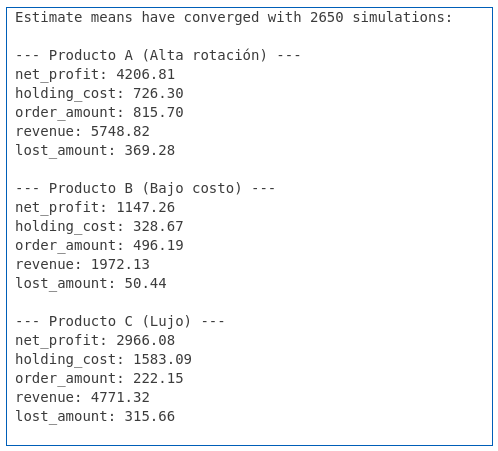
\includegraphics[scale=0.4, keepaspectratio]{images/1.png}
            \caption{Ganancia neta promedio de cada producto}
            \label{fig:ganancia}
        \end{figure}

        \begin{figure}[H] 
            \centering
            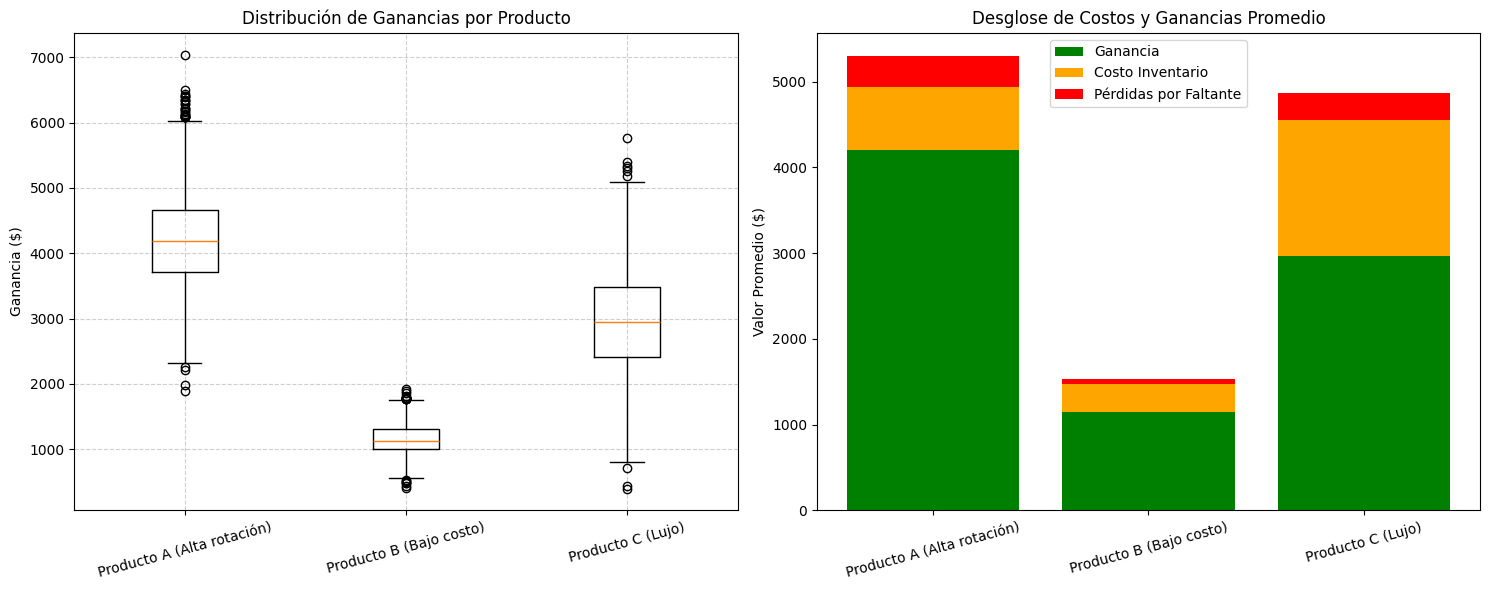
\includegraphics[scale=0.4, keepaspectratio]{images/2.png}
            \caption{Graficación de la ganancia neta promedio}
            \label{fig:ganancia_graficacion}
        \end{figure}

        \begin{figure}[H] 
            \centering
            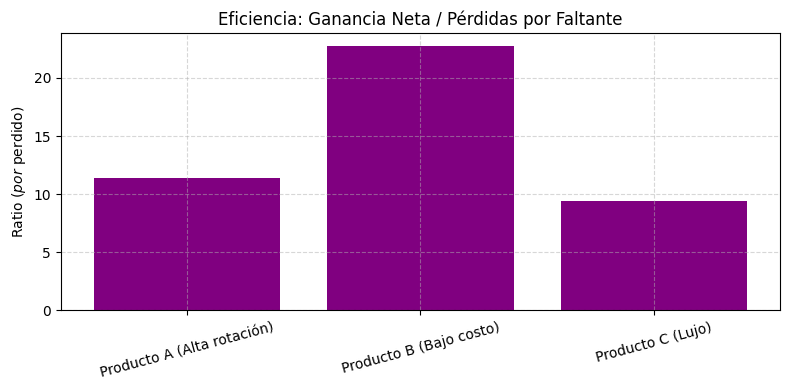
\includegraphics[scale=0.4, keepaspectratio]{images/3.png}
            \caption{Eficiencia por producto}
            \label{fig:eficiencia}
        \end{figure}

        Y entonces podemos llegar a las siguentes conclusiones: 

        \vspace*{0.5cm}

        \textbf{Producto A (Alta rotación)}

        El producto A, caracterizado por su alta frecuencia de ventas, mostró una ganancia neta promedio de \textbf{\$4206.81}, con un ingreso promedio de \textbf{\$5748.82}. Este desempeño positivo se acompaña de un costo de inventario moderado de \textbf{\$726.30} y pérdidas por faltantes por un valor promedio de \textbf{\$369.28}. La alta rotación del producto permite una ganancia destacada, aunque las pérdidas por faltante todavía representan un valor no despreciable, lo que indica oportunidad de mejora en la política de reabastecimiento para reducir estas pérdidas.

        \vspace*{0.5cm}

        \textbf{Producto B (Bajo costo)}

        El producto B, de bajo costo y menor margen unitario, obtuvo una ganancia neta promedio de \textbf{\$1147.26}. Aunque modesta en comparación con los otros productos, presenta el ratio de eficiencia más alto (ganancia por cada dólar perdido), lo que sugiere que su política de inventario ha sido especialmente eficiente. Las pérdidas por faltante fueron mínimas (\textbf{\$50.44}), con un costo de inventario también reducido (\textbf{\$328.67}), lo que refuerza su comportamiento estable dentro del portafolio.

        \vspace*{0.5cm}

        \textbf{Producto C (Lujo)}

        El producto C, de categoría de lujo y menor frecuencia de compra, alcanzó una ganancia neta promedio de \textbf{\$2966.08}, con ingresos por \textbf{\$4771.32}. A pesar de estos buenos números, el producto presenta un costo de inventario elevado (\textbf{\$1583.09}) y pérdidas por faltante significativas (\textbf{\$315.66}), lo que podría estar asociado a una alta variabilidad en la demanda o a una política de inventario más conservadora. Es recomendable analizar si estos costos podrían optimizarse sin afectar los ingresos.

    \subsection{¿Qué producto es más afectado por cambios en la demanda?}

        Con el objetivo de comprender cómo la ganancia neta se ve influenciada por cambios en la demanda, se llevó a cabo un nuevo experimento simulando distintos escenarios de demanda promedio (\texttt{demand\_mean}). A diferencia del modelo anterior, donde la demanda se generaba usando una distribución de Poisson, en este análisis se optó por una distribución \textbf{normal truncada en cero}, con media variable y desviación estándar fija. Esta elección permite explorar de forma más continua y realista el impacto de diferentes niveles promedio de demanda sobre las ganancias.

        Para cada valor de \texttt{demand\_mean} en el rango $[2, 4, 6, 8, 10, 12, 14]$, se ejecutaron simulaciones estocásticas hasta alcanzar convergencia en la ganancia promedio estimada (\texttt{net\_profit}). El criterio de parada fue el mismo que en análisis anteriores: se aumentó progresivamente el número de simulaciones hasta que el intervalo de confianza al 95\,\% para la ganancia tuviera una amplitud menor a 30 dólares.

        \begin{figure}[H] 
            \centering
            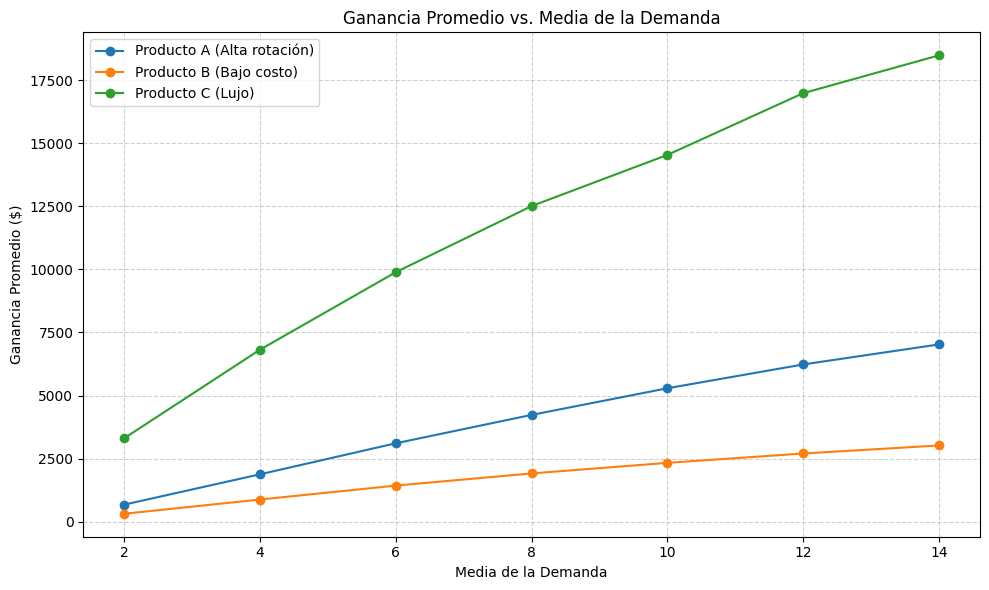
\includegraphics[scale=0.4, keepaspectratio]{images/4.png}
            \caption{Ganancia neta promedio por producto en función de la demanda promedio}
            \label{fig:demanda}
        \end{figure}

        Los resultados, presentados en la Figura ~\ref{fig:demanda}, muestran que \textbf{las ganancias aumentan consistentemente con la demanda promedio}, como era de esperarse. No obstante, el crecimiento no es igual para todos los productos. El \textbf{Producto C (Lujo)} presenta el mayor incremento absoluto en ganancias a medida que crece la demanda, seguido por el \textbf{Producto A (Alta rotación)}. En cambio, el \textbf{Producto B (Bajo costo)}, aunque también crece, lo hace de forma más moderada. Esto sugiere que productos con mayor margen unitario o mayor precio de venta se benefician más intensamente del aumento en la demanda.

        \subsection{¿Qué pasa si cambian los precios de venta?}

        Con el propósito de estudiar cómo afectan las variaciones en los precios de venta a la rentabilidad de cada producto, se realizó una simulación modificando los valores de \texttt{sell\_price} en un rango controlado. El resto de parámetros del sistema, incluyendo demanda, costos y políticas de reabastecimiento, se mantuvieron constantes.
        
        Se probaron diferentes precios para cada producto, variando desde un 60\,\% hasta un 200\,\% del precio base, en pasos del 20\,\%. Por cada combinación, se ejecutaron simulaciones estocásticas hasta que la estimación de la \textbf{ganancia neta promedio} (\texttt{net\_profit}) alcanzara convergencia, bajo el mismo criterio de precisión utilizado anteriormente (intervalo de confianza al 95\,\% con amplitud menor a 30 dólares).
        
        \begin{figure}[H] 
            \centering
            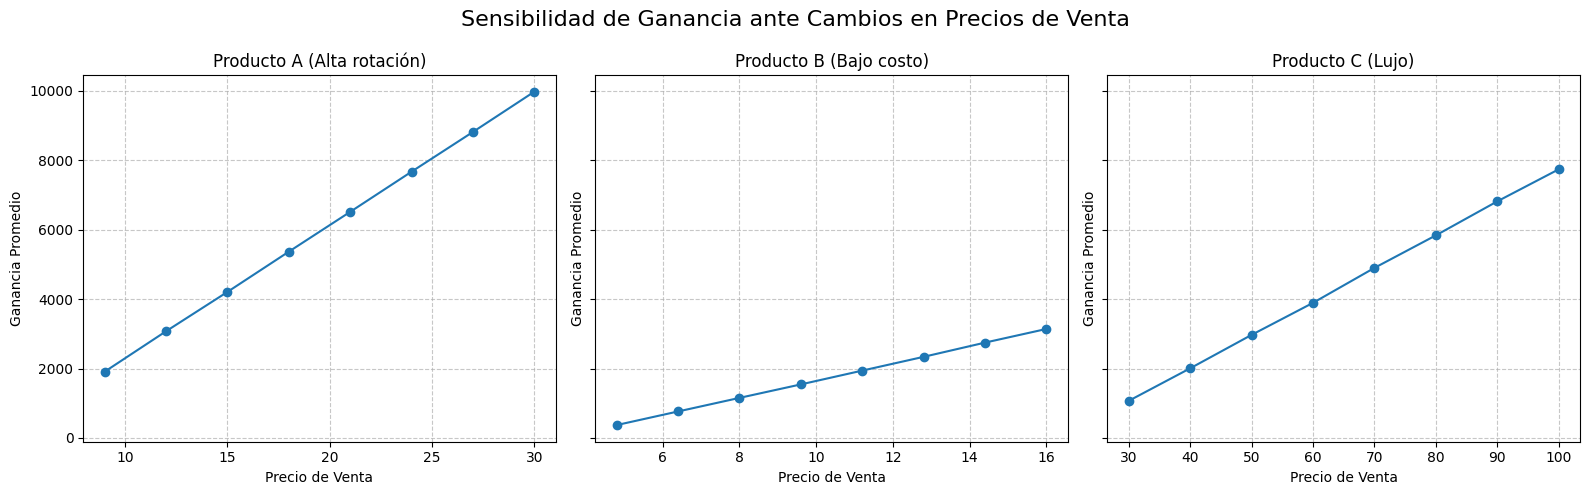
\includegraphics[scale=0.4, keepaspectratio]{images/5.png}
            \caption{Ganancia neta promedio por producto en función del precio de venta}
            \label{fig:precios}
        \end{figure}

        Los resultados de la Figura~\ref{fig:precios} muestran que:
        
        \begin{itemize}
            \item \textbf{Producto A (Alta rotación)}  
            Es el más sensible a los aumentos de precio. Su ganancia crece de forma pronunciada, lo que indica una alta \textbf{elasticidad de ingresos} positiva en este rango. Probablemente tiene una demanda estable, lo cual permite subir precios sin afectar tanto las ventas.
        
            \item \textbf{Producto B (Bajo costo)}  
            Tiene una curva mucho más plana, lo que indica que su ganancia \textbf{no varía tanto} con los cambios en el precio de venta. Esto sugiere que tiene un margen ajustado o que su demanda es más sensible, haciendo que los ingresos adicionales por precio no compensen tanto los costos o la pérdida de volumen.
        
            \item \textbf{Producto C (Lujo)}  
            Aumenta también de manera constante, aunque con una pendiente menor que A pero mayor que B. Esto puede indicar que tiene algo de margen para aumentar precios sin perder rentabilidad, pero no tanto como A. Su demanda podría ser más estable debido a su segmento de lujo.
        \end{itemize}
        
        Este análisis permite identificar el rango de precios que maximiza la ganancia para cada producto, revelando así su \textbf{elasticidad de ingresos}. Ajustar precios dentro de ese rango puede mejorar la rentabilidad sin comprometer significativamente el volumen de ventas.
    

        
\newpage

\section{Modelo Matemático}\label{S4}
\subsection{Descripción del modelo}
Presentación del modelo matemático utilizado, incluyendo modelos probabilísticos si aplica...

\subsection{Supuestos y restricciones}
\begin{itemize}
    \item Supuesto 1
    \item Supuesto 2
    % Añade más supuestos según sea necesario
\end{itemize}

\subsection{Comparación de resultados}
Análisis comparativo entre los resultados obtenidos y los resultados experimentales...

\section{Conclusiones}\label{S5}
Resumen de los principales hallazgos y conclusiones del proyecto...

\begin{itemize}
    \item Conclusión 1
    \item Conclusión 2
    % Añade más conclusiones según sea necesario
\end{itemize}

\end{document}